\chapter{Erweiterte Funktionen}
In diesem Kapitel werden nun Funktionen beschrieben, die über die Grundausstattung der Web-App hinaus gehen, um diese zu erweitern und produktiver zu gestalten. 

\section{Statistiken}
Da eine Auswertung der eingegebenen Daten für Veranstaltungen unabdinglich ist, wurde ein weiterer Controller implementiert, welcher sämtliche speziellen Felder der Events aus der Datenbank abfragt und diesen dann die Werte der einzelnen Benutzer zuweist.\par

Im View wird dann eine grafische Auswertung gestartet, die mit Hilfe von Google Charts ansehnliche Graphen generiert, bei denen es Sinn ergibt und vergleichbare Werte von den Benutzern hinterlegt wurden. Außerdem gibt es allgemeine Statistiken, die die Veranstaltungen untereinander vergleichen, durch JavaScript gestützte Graphen visualisiert.

\section{Lokalisierung von Clients}
Um die eingetragenen Helfer in dieser Webanwendung besser koordinieren zu können, wurde ein Modul implementiert, welches im Hintergrund der Web-App läuft und die aktuelle Position des Endgeräts über eine SSL verschlüsselte Verbindung an den Server übermittelt. Unter der Voraussetzung, dass der Client diesem Vorgang zustimmt, sind dem Server damit die Positionen der eingeloggten Benutzer bekannt. Diese Positionsdaten können dann von der Anwendung ausgewertet und in einer Karte von Google Maps angezeigt werden.\par

Jeder Client kann auf diese Weise die Positionen der anderen Helfer sehen. Der Vorteil liegt klar auf der Hand: eine zentral eingerichtete Verwaltung kann mit einem Blick sehen, wer sich an welcher Stelle auf dem Gelände befindet. So können Wege optimiert und gezielt Aufgaben verteilt werden, da ortsnahe Helfer die entsprechenden Aufgaben übernehmen können. Die kurzen Wege sorgen dann dafür, dass eine höhere Nutzung der Ressourcen (hier: die Helfer) möglich ist.\par

Eine wichtige Anforderung ist außerdem, dass die Daten schnell ausgetauscht werden. Wenn zwischen den Updates der Positionen zu viel Zeit vergeht, ist die aktuelle Position nicht mehr aktuell und damit nicht mehr relevant.\par

Wie findet der Austausch der Positionen denn nun statt? Da es sich hier um sensible Daten handelt, ist eine sichere Übertragung Grundvoraussetzung. Allerdings steht im W3C Working Draft, dass keine sichere, verschlüsselte Peer to Peer Verbindung mit HTML5 möglich ist \cite{w3cworkingdraft}. Im aktuellen Draft wurde auch keine sichere Verbindung definiert und es ist auch bisher keine vorgesehen \cite{w3ccurrent}.\\
Also liegt nahe weitere Techniken zu betrachten, welche einen sicheren Austausch von Daten zwischen Clients über einen Server ermöglichen.

\section{Echtzeitaktualisierung durch WebSockets}
Das wohl spannendste Thema dieser Arbeit ist die Echtzeitaktualisierung im Hintergrund der Web-App. Mehrere Möglichkeiten sind dafür gegeben, wobei einige besser geeignet sind als andere.

\subsection{Vor HTML5: Benutzung von Polling}
Für den Datenverkehr von Internetseiten wird HTTP benutzt, welches die wechselseitige Datenübermittlung \emph{Halbduplex} verwendet. So erfolgt der Datenverkehr nur in eine Richtung zur gleichen Zeit. Der Client schickt eine Anfrage an den Server und dieser übermittelt danach die Antwort \cite[S. xx]{ws}. Das hat wiederum zur Folge, dass es relative ineffizient ist, da man mit jeder Anfrage stets die Antwort des Servers abwarten muss und gleichzeitig Übertragungen nicht möglich sind.\par

Vor diesem technischen Hintergrund wurde Polling entwickelt, bei dem in einem zeitlich bekannten Intervall eine Anfrage an den Server geschickt wurde mit der Bitte um Aktualisierung. Diese Technik ist sehr attraktiv, wenn die zeitlichen Abstände der Aktualisierung der Daten bekannt ist, allerdings sind Echtzeitdaten schlecht vorhersagbar. Dadurch ist Polling nicht die richtige Wahl für dieses Projekt, da es auf eine wirkliche Echtzeitaktualisierung ankommt.\par

\subsection{Einführung in WebSockets}
Mit der HTML5-Spezifikation wurden \emph{WebSockets} eingeführt, welche eine Vollduplex, bidirektionale, Single-Socket Verbindung ermöglichen \cite[S. Introducing WebSocket]{ws}. Eine Anfrage öffnet die Verbindung zum WebSocket Server und kann beliebig lange offen gehalten werden, wobei zu jeder Zeit Daten zwischen Client und Server ausgetauscht werden. Dieser erste Handshake erfolgt über HTTP/1.1 und ähnelt dem zum Aufruf einer Homepage.
\\
\begin{lstlisting}[captionpos=b, caption=HTTP Request vom Client {\cite[S. 6]{rfc6455:handshake}}]
  GET / HTTP/1.1
  Host: server.example.com
  Origin: http://www.example.com
  Sec-WebSocket-Key: 7+C600xYyb0v2zmJ69RQsw==
  Sec-WebSocket-Version: 13
  Upgrade: websocket
\end{lstlisting}

Mit \emph{Upgrade: websocket} wird signalisiert, dass der Client eine WebSocket-Verbindung zum Server aufbauen möchte. Der entsprechende WebSocket Server reagiert darauf mit dem HTTP-Statuscode \emph{101 Switching Protocols}, womit er bestätigt, dass er mit dem Wechsel des Protokolls einverstanden ist.
\\
\begin{lstlisting}[captionpos=b, caption=HTTP Response vom Server {\cite[S. 8]{rfc6455:handshake}}]
  101 Switching Protocols
  Connection: Upgrade
  Sec-WebSocket-Accept: fYoqiH14DgI+5y1EMwM2sOLzOi0=
  Upgrade: WebSocket
\end{lstlisting}

Der kryptische Schlüssel \emph{Sec-WebSocket-Accept} muss vom Server berechnet und zurückgegeben werden und zeigt damit, dass er das WebSocket Protokoll versteht.

\begin{figure}[!ht]
	\centering
	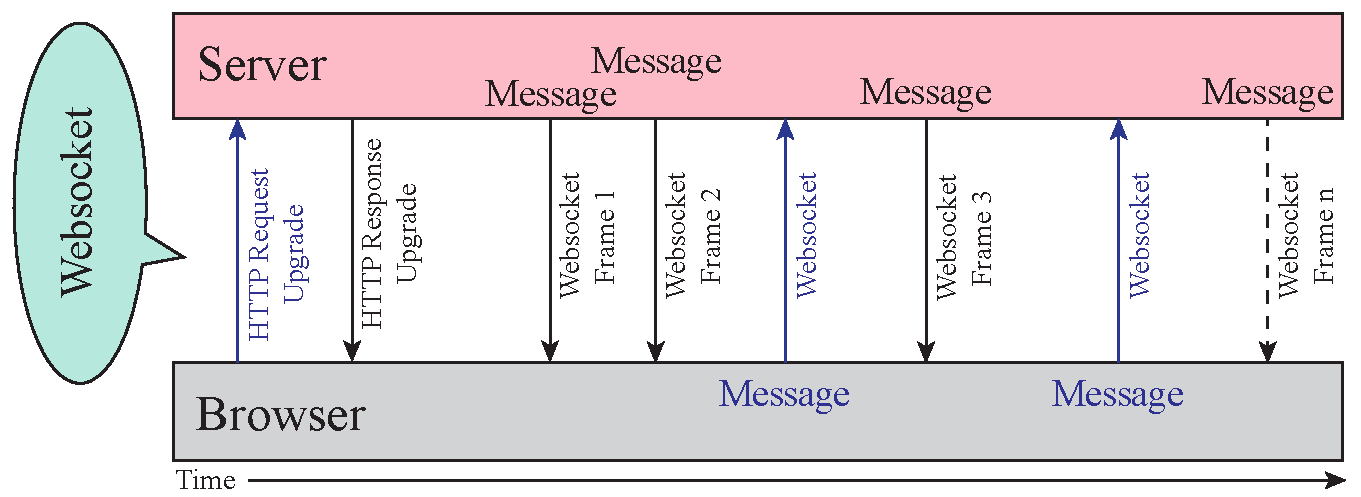
\includegraphics[width=15cm]{fig/websockets}
	\caption{Aufbau einer WebSocket Verbindung. Danach können beliebig (auch gleichzeitig) in beide Richtungen Nachrichten übermittelt werden}
\end{figure}
























